\documentclass[10pt,a4paper,twocolumn]{article}

% Modelo-base para Overleaf. Conferir o manual da UCDB antes da entrega.
\usepackage[utf8]{inputenc}
\usepackage[T1]{fontenc}
\usepackage[brazil]{babel}
\usepackage{lmodern}
\usepackage{microtype}
\usepackage[a4paper,top=1.45cm,bottom=1.55cm,left=1.35cm,right=1.35cm,columnsep=0.62cm]{geometry}
\usepackage{setspace}
\usepackage{graphicx}
\usepackage{booktabs}
\usepackage{tabularx}
\usepackage{array}
\usepackage{float}
\usepackage{amsmath}
\usepackage{listings}
\usepackage{xcolor}
\usepackage{url}
\usepackage{hyperref}
\usepackage{tikz}
\usetikzlibrary{arrows.meta,positioning,shapes.geometric,fit,calc}
\usepackage{dblfloatfix}
\usepackage{balance}
\usepackage[numbers,sort&compress]{natbib}

\hypersetup{
  colorlinks=true,
  linkcolor=black,
  citecolor=black,
  urlcolor=blue,
  pdftitle={Blockchain pública e privada em ambientes IoT},
  pdfauthor={João Henrique Schweitzer Rezende; Luan Henrique Santos Miranda; Alexandre dos Santos Batista}
}
\setstretch{1.0}
\setlength{\parindent}{0.45cm}
\setlength{\parskip}{0.02em}
\renewcommand{\arraystretch}{1.12}\setlength{\columnsep}{0.62cm}\setlength{\emergencystretch}{2em}

\lstdefinestyle{codigo}{
  basicstyle=\ttfamily\small,
  breaklines=true,
  frame=single,
  numbers=left,
  numberstyle=\tiny,
  showstringspaces=false,
  tabsize=4
}

\title{Blockchain Pública e Privada em Ambientes IoT: Análise Comparativa entre Ethereum e Hyperledger Fabric e Implementação de um Protótipo de Blockchain Privada para Integridade e Rastreabilidade de Dados}
\author{João Henrique Schweitzer Rezende\thanks{E-mail: ra189395@ucdb.br}, Alexandre dos Santos Batista\thanks{E-mail: rf1588@ucdb.br}\\[0.35em]\small Universidade Católica Dom Bosco (UCDB), Campo Grande -- MS, Brasil}
\date{}

\begin{document}
\twocolumn[
\begin{minipage}{\textwidth}
\centering
{\large\bfseries Blockchain Pública e Privada em Ambientes IoT: Análise Comparativa entre Ethereum e Hyperledger Fabric e Implementação de um Protótipo de Blockchain Privada para Integridade e Rastreabilidade de Dados\par}
\vspace{0.65em}
{\small Universidade Católica Dom Bosco (UCDB), Campo Grande -- MS, Brasil\par}
\vspace{0.45em}
{\footnotesize João Henrique Schweitzer Rezende\textsuperscript{1}, Alexandre dos Santos Batista\textsuperscript{1}\par}
\vspace{0.25em}
{\scriptsize \textsuperscript{1}E-mails: ra189395@ucdb.br; rf1588@ucdb.br\par}
\vspace{0.8em}
\hrule
\vspace{0.55em}
\begin{minipage}{0.97\textwidth}
\small
\noindent\textbf{Resumo.} A Internet das Coisas (IoT) exige mecanismos para verificar autoria, integridade e rastreabilidade de leituras. Este trabalho compara bibliograficamente Ethereum e Hyperledger Fabric e avalia um protótipo local em Python. A versão atual contém transações e blocos assinados com Ed25519, hashes SHA-256, cadastro versionado de identidades, prevenção de reenvio de transações, cofre de chaves cifradas, persistência SQLite, API HTTP local, simulador de sensores e painel web. Em 2 de novembro de 2026, uma cópia da distribuição foi instalada em Windows com Python 3.15.1 e os 113 testes automatizados foram aprovados. Uma execução HTTP confirmou duas leituras simuladas em um bloco, detectou adulteração em cópia e recuperou o histórico íntegro após reiniciar o servidor. A avaliação quantitativa arquivada, realizada anteriormente com Python 3.12.14, compreende 24 execuções: 200 ou 600 leituras, lotes de 10 ou 50 e três repetições por cenário em dois modos, ledger e controle SQLite. O throughput médio do ledger variou de 61,31 a 675,37 leituras confirmadas por segundo nas cargas medidas. O controle SQLite executou um conjunto menor de verificações e obteve taxas superiores. Os experimentos não mediram HTTP, painel, sensores físicos ou redes Ethereum/Fabric. O protótipo opera em um único processo, com rodízio local entre autoridades; não possui consenso distribuído nem replicação. Assinaturas comprovam vínculo com uma chave, mas não a veracidade física das leituras.\par

\vspace{0.45em}
\noindent\textbf{Palavras-chave:} Blockchain; Internet das Coisas; Ethereum; Hyperledger Fabric; integridade; rastreabilidade; Ed25519; Proof of Authority; problema do oráculo.
\end{minipage}
\vspace{0.6em}
\hrule
\vspace{0.8em}
\end{minipage}
]
\section{Introdução}
A Internet das Coisas (IoT) conecta dispositivos físicos capazes de coletar, processar e transmitir dados em diferentes contextos, incluindo automação industrial, monitoramento ambiental, logística, saúde e edifícios inteligentes. A distribuição dos dispositivos amplia a disponibilidade de informações, mas também cria desafios relacionados à identidade dos emissores, à integridade dos registros, à auditoria e à confiança entre organizações. A literatura identifica tanto oportunidades de integração entre IoT e blockchain quanto restrições de custo computacional, latência, largura de banda e privacidade \cite{Christidis2016,Dorri2017,Pajooh2022}.

Blockchain é uma estrutura de registro em que os dados são organizados em blocos vinculados criptograficamente e sujeitos a regras de validação. Em arquiteturas distribuídas, cópias do registro são mantidas por participantes da rede; o nível de descentralização e a resistência a falhas dependem do protocolo e das suposições de confiança adotadas \cite{Nakamoto2008,Yaga2018}. Consequentemente, o uso de blockchain não garante, por si só, que uma leitura de sensor seja verdadeira: um dado incorreto pode ser registrado com integridade caso a origem esteja comprometida ou produza informação errada.

Este trabalho investiga a adequação de duas plataformas com modelos de governança distintos: Ethereum, uma plataforma pública baseada em execução de contratos inteligentes, e Hyperledger Fabric, uma plataforma permissionada voltada a redes cujos participantes são conhecidos e autorizados \cite{Wood2014,Androulaki2018}. A comparação considera requisitos de integridade e rastreabilidade em cenários IoT e é complementada pelo desenvolvimento de uma prova de conceito em Python.

\subsection{Problema de pesquisa}
A questão principal é: \textit{quais diferenças arquiteturais entre Ethereum e Hyperledger Fabric influenciam sua adequação a aplicações IoT que exigem integridade, rastreabilidade, controle de acesso e desempenho?} Como questão complementar, investiga-se em que medida um protótipo didático em Python consegue demonstrar mecanismos verificáveis de assinatura, encadeamento de hashes e validação de registros, e quais limitações permanecem em comparação com uma blockchain distribuída.

\subsection{Objetivos}
O objetivo geral é comparar Ethereum e Hyperledger Fabric para cenários IoT e desenvolver um protótipo didático que demonstre mecanismos básicos de integridade e rastreabilidade.

Os objetivos específicos são:
\begin{itemize}
  \item caracterizar os modelos de arquitetura, identidade, privacidade e validação das duas plataformas;
  \item sintetizar evidências da literatura sobre desempenho e escalabilidade, explicitando diferenças de ambiente experimental;
  \item implementar estruturas de transações e blocos com hashes encadeados, assinaturas digitais e persistência;
  \item avaliar por testes funcionais a detecção de adulterações e a rejeição de transações inválidas;
  \item medir throughput e latência em cargas locais controladas, distinguindo o ledger de um controle SQLite com garantias diferentes;
  \item discutir limitações de segurança, governança, privacidade e validade externa dos resultados.
\end{itemize}

\subsection{Contribuições e delimitação}
As contribuições são: (i) a comparação bibliográfica entre Ethereum e Hyperledger Fabric; (ii) um protótipo Python com identidade versionada, assinaturas, encadeamento, recuperação, API e painel; (iii) uma suíte funcional de 113 testes aprovada na versão distribuída; e (iv) 24 execuções experimentais locais arquivadas, com cargas e ambiente documentados. As medições foram feitas sobre as fontes preservadas da etapa experimental, anteriores à reorganização de diretórios; não constituem novas medições da distribuição reorganizada. O sistema opera em um único processo, sem P2P, replicação, consenso distribuído, tolerância a falhas de nós ou contratos inteligentes programáveis. Os resultados não medem Ethereum ou Fabric e não comprovam desempenho ou segurança de uma rede de produção.

\section{Fundamentação teórica}
\subsection{Blockchain, hashes e assinaturas digitais}
O SHA-256 é uma função hash padronizada que mapeia uma entrada de tamanho arbitrário para uma saída de tamanho fixo. Em condições apropriadas, pequenas alterações na entrada produzem saídas distintas, permitindo detectar modificações no conteúdo \cite{FIPS1804}. O encadeamento ocorre quando cada bloco inclui o hash do bloco anterior; uma alteração em bloco anterior invalida o encadeamento subsequente, desde que a validação percorra a cadeia e compare os valores calculados \cite{Nakamoto2008,Yaga2018}.

Assinaturas digitais permitem verificar se uma mensagem foi assinada com a chave privada correspondente a uma chave pública. O Ed25519 é um esquema de assinatura digital baseado em curvas elípticas, especificado no RFC 8032 \cite{Josefsson2017}. No protótipo, SHA-256 é usado para calcular hashes e Ed25519 para assinar e verificar transações. Essas primitivas são utilizadas por bibliotecas consolidadas; não são implementadas do zero \cite{CryptographyEd25519}.


A função hash não cifra o conteúdo e não deve ser interpretada como mecanismo de sigilo. O hash permite verificar se a representação analisada corresponde ao resumo criptográfico esperado, mas não impede que alguém autorizado leia o dado original. Da mesma forma, uma assinatura digital não torna o dado confidencial: ela permite verificar autoria e integridade relativamente à chave pública usada na verificação. Para confidencialidade, seriam necessários controles adicionais, como criptografia, gestão de chaves e políticas de acesso. Essa distinção é particularmente importante em IoT, onde uma leitura pode conter informação operacional sensível ou até revelar hábitos de pessoas quando correlacionada com outros dados.

A serialização faz parte da segurança do sistema. Se dois nós representarem o mesmo objeto JSON com ordenações, espaços, codificações ou tipos numéricos diferentes, poderão calcular hashes distintos. Por isso, uma implementação precisa definir uma representação canônica e consistente para os campos assinados. No protótipo, a função \texttt{canonico} usa JSON com chaves ordenadas, separadores compactos e codificação UTF-8. Essa solução é adequada à demonstração controlada, mas ainda exige disciplina na validação de entradas, na normalização de valores, no tratamento de números e na definição de versões do formato quando o sistema evoluir.

\subsection{Estrutura de blocos e encadeamento criptográfico}
Um bloco de blockchain costuma combinar metadados de posição, referência ao bloco anterior e um conjunto de transações. O encadeamento estabelece uma dependência entre os blocos: o bloco de índice $i$ armazena o hash do bloco $i-1$. Durante a validação, o software recalcula o hash a partir do conteúdo disponível e compara o resultado com o valor armazenado. Se um campo protegido for modificado sem atualizar o hash, a divergência é detectada. Se o hash for recalculado, a alteração ainda pode ser detectada por assinaturas digitais associadas ao conteúdo original, desde que a assinatura e o vínculo entre os campos sejam corretamente verificados.

A Figura~\ref{fig:encadeamento} representa essa relação. Ela mostra a dependência entre os blocos, mas não implica, por si só, descentralização. Um arquivo local com vários blocos encadeados também pode implementar essa estrutura; para constituir uma blockchain distribuída são necessários participantes independentes, regras comuns para aceitar novos registros e algum mecanismo de consenso ou coordenação entre eles \cite{Yaga2018,Zheng2017}.

\begin{figure*}[t]
\centering
\begin{tikzpicture}[
  bloco/.style={draw,rounded corners=2pt,minimum width=4.15cm,minimum height=1.55cm,align=center,font=\small},
  seta/.style={-{Stealth[length=2.4mm]},thick},
  node distance=1.25cm]
  \node[bloco] (b0) {\textbf{Bloco $i-1$}\\Transações e metadados\\Hash anterior: $H_{i-2}$\\Hash calculado: $H_{i-1}$};
  \node[bloco,right=of b0] (b1) {\textbf{Bloco $i$}\\Transações e metadados\\Hash anterior: $H_{i-1}$\\Hash calculado: $H_i$};
  \node[bloco,right=of b1] (b2) {\textbf{Bloco $i+1$}\\Transações e metadados\\Hash anterior: $H_i$\\Hash calculado: $H_{i+1}$};
  \draw[seta] (b0.east) -- (b1.west);
  \draw[seta] (b1.east) -- (b2.west);
  \node[below=0.55cm of b1,align=center,font=\small,text width=13cm] {Alterar o conteúdo de um bloco modifica o hash recalculado. A divergência pode ser detectada ao validar o bloco e os vínculos subsequentes.};
\end{tikzpicture}
\caption{Modelo conceitual de encadeamento dos blocos por hashes criptográficos. Fonte: elaboração própria, com base em \cite{Nakamoto2008,Yaga2018}.}
\label{fig:encadeamento}
\end{figure*}

\subsection{Consenso, ordenação e finalidade}
O consenso é o conjunto de regras que permite a participantes distribuídos concordarem sobre quais transações e blocos compõem o histórico válido. A criptografia contribui para identificar conteúdo e autoria, mas não substitui o consenso: assinaturas válidas podem existir em blocos conflitantes, e um conjunto de participantes ainda precisa decidir qual sequência aceitar. Os requisitos variam conforme a rede aberta ou permissionada e conforme as falhas que o protocolo pretende tolerar.

O Proof of Work (PoW) seleciona produtores de blocos por competição computacional. A segurança econômica depende do custo de controlar o poder de mineração, mas o mecanismo exige consumo de energia e pode oferecer finalidade probabilística. O Proof of Stake (PoS) associa a participação na validação a um depósito econômico sujeito a penalidades. O Ethereum migrou para PoS em 2022; sua operação usa slots de 12 segundos e épocas compostas por 32 slots, e a finalidade resulta de votações de validadores sobre checkpoints, não de uma regra simples baseada apenas em aguardar um número fixo de blocos \cite{EthereumDocs}. Assim, explicações sobre Ethereum precisam distinguir a rede atual de descrições históricas baseadas em mineração PoW.

Em blockchains permissionadas, os participantes são conhecidos ou certificados e a governança define quem pode propor, ordenar ou validar transações. O Hyperledger Fabric separa execução/endorsement, ordenação e validação/commit. A ordenação organiza a sequência de transações, mas uma transação ainda precisa passar pelas verificações de validade correspondentes antes de ser considerada comprometida no ledger. O serviço de ordenação pode ser configurado com protocolos diferentes. Raft oferece tolerância a falhas por queda de nós (Crash Fault Tolerance, CFT), enquanto configurações baseadas em SmartBFT visam tolerância a falhas bizantinas; a disponibilidade de opções depende da versão e da configuração efetivamente implantadas \cite{Androulaki2018,FabricDocs}.

O Proof of Authority (PoA) costuma representar uma rede em que a produção de blocos fica reservada a autoridades previamente autorizadas. Essa designação não identifica um único protocolo universal: as regras de seleção, rotação, votação, tolerância a falhas e recuperação variam por implementação. No protótipo deste trabalho, o termo PoA designa apenas uma regra determinística local: para cada índice, o produtor deve ser o nome esperado no rodízio. Como não existem réplicas concorrentes nem troca de mensagens, a regra comprova o cumprimento de uma condição programada, mas não resolve conflitos entre nós independentes.

A integridade criptográfica deve ser distinguida da veracidade semântica. A assinatura confirma a associação entre uma mensagem e uma chave, mas não prova que o sensor mediu corretamente o fenômeno físico. Esse limite é conhecido como problema do oráculo em sistemas que registram dados externos \cite{Christidis2016,Yaga2018}.

\subsection{Blockchain pública e permissionada}
Redes públicas permitem participação e verificação por um conjunto amplo de agentes, ainda que as operações e os mecanismos de consenso estejam sujeitos às regras do protocolo. Ethereum utiliza execução de contratos inteligentes e, atualmente, consenso Proof of Stake; a finalidade do protocolo não deve ser confundida com uma regra simplificada de número fixo de confirmações \cite{Wood2014,EthereumDocs}.

Redes permissionadas restringem a participação a identidades conhecidas e podem estabelecer políticas de acesso, canais de privacidade e governança organizacional. O Hyperledger Fabric separa etapas de proposta, ordenação e validação das transações, além de permitir políticas de endosso e controle de identidade \cite{Androulaki2018,FabricDocs}. Portanto, a confirmação de uma transação no Fabric não deve ser descrita apenas como o momento em que um serviço de ordenação recebe ou organiza a transação: o fluxo inclui validação e registro pelos peers.


\subsection{Ethereum: execução, incentivos e auditabilidade pública}
Ethereum é uma plataforma pública cujo estado é atualizado por transações executadas de acordo com as regras do protocolo. O uso de contratos inteligentes permite descrever regras verificáveis no estado compartilhado, incluindo validação de condições, registro de eventos e interação entre aplicações. A execução é determinística para uma mesma sequência de transações válidas e o mesmo estado anterior; por isso, todos os nós que verificam a mesma cadeia podem reproduzir as transições de estado. A execução de um contrato, entretanto, não faz com que os dados externos se tornem verdadeiros: um contrato que depende de uma leitura de temperatura precisa receber esse valor de uma fonte externa e continua sujeito ao problema do oráculo.

A auditabilidade pública constitui uma vantagem quando organizações, clientes ou reguladores precisam verificar o histórico sem depender de uma permissão concedida por um operador único. Em contrapartida, os dados incluídos em transações públicas podem ser observados e correlacionados. Pseudonimato não equivale a anonimato, pois os endereços e metadados podem ser associados a pessoas ou organizações por informações auxiliares. Para aplicações IoT, a publicação de cada leitura bruta pode elevar custos, expor padrões operacionais e gerar um volume de transações pouco compatível com a frequência de sensores. Estratégias híbridas podem manter os dados detalhados fora da cadeia e ancorar na blockchain apenas hashes, referências ou eventos cuja publicação seja justificada.

O custo de execução em Ethereum é expresso por gas e, na rede pública, resulta em taxas pagas conforme as regras da plataforma e as condições de mercado. Esse custo precisa integrar o projeto econômico de uma aplicação IoT contínua, na qual sensores podem gerar leituras frequentes. As taxas e o congestionamento não devem, contudo, ser tratados como atributos imutáveis de todas as redes baseadas em Ethereum: redes privadas compatíveis com a EVM têm modelos de governança e configuração diferentes, e os resultados de desempenho de uma implantação privada não podem ser automaticamente atribuídos à mainnet pública.

\subsection{Hyperledger Fabric: identidade, políticas e privacidade}
O Hyperledger Fabric foi concebido para redes permissionadas em que organizações participantes administram suas identidades e políticas de colaboração. A arquitetura separa responsabilidades, permitindo que os peers mantenham o ledger e executem chaincode, que o serviço de ordenação estabeleça a sequência de blocos e que políticas de endosso determinem quais organizações ou peers precisam aprovar uma proposta. A separação facilita a configuração de regras de negócio em redes empresariais, mas aumenta a importância da modelagem de governança, certificados, canais, políticas e administração operacional \cite{Androulaki2018,FabricDocs}.

A infraestrutura de identidade pode usar certificados digitais e provedores de serviço de membros. Isso permite associar ações a organizações e identidades gerenciadas, ao contrário do pseudonimato típico de endereços em redes públicas. Canais fornecem ledgers segregados para subconjuntos de organizações, enquanto coleções de dados privados podem restringir certos dados a membros autorizados, conforme a configuração. Essas estruturas ajudam a reduzir a exposição, mas não eliminam a necessidade de classificar dados, gerenciar chaves, definir retenção e registrar acessos.

O modelo de execução e validação do Fabric também afeta o desempenho. Uma proposta pode passar por endosso dos peers relevantes, ordenação e validação/commit. A quantidade de endossos exigidos, o tamanho dos blocos, a política de leitura/escrita, a distribuição dos peers e o volume de contendas por estado alteram a latência. Uma política mais rigorosa pode melhorar a governança e a segurança, mas acrescentar comunicação e trabalho de validação. Por isso, o número de transações por segundo não deve ser citado isoladamente sem identificar a carga utilizada e o procedimento de confirmação.

\subsection{Modelos de governança e decisão de adoção}
A escolha entre uma rede pública e uma permissionada deve começar pela pergunta sobre a necessidade real de blockchain. Se existe um único escritor confiável e um operador responsável pela auditoria, um banco de dados convencional pode ser mais simples, barato e facilmente governável. Se há múltiplos escritores, mas as organizações confiam umas nas outras e aceitam um administrador comum, um banco replicado com trilha de auditoria também pode atender ao requisito. Uma blockchain permissionada torna-se mais justificável quando múltiplas organizações precisam manter um registro compartilhado, com identidades conhecidas, e não querem conceder controle exclusivo a uma única delas. Uma blockchain pública ganha relevância quando a participação aberta e a verificabilidade por terceiros não credenciados são requisitos centrais \cite{WuestGervais2018,Yaga2018}.

A matriz da Tabela~\ref{tab:decisao} resume a lógica de decisão e busca evitar que a blockchain seja escolhida apenas por ser uma tecnologia emergente. Ela não prescreve uma plataforma única: registra critérios que precisam ser respondidos antes da escolha. Em sistemas IoT, a frequência dos dados, o custo por gravação, a capacidade de armazenamento e a tolerância a atraso devem ser somados ao modelo de confiança para que uma alternativa tecnicamente correta também seja sustentável no uso real.

\begin{table*}[t]
\centering\small
\caption{Critérios de decisão para selecionar a arquitetura de registro em aplicações IoT.}
\label{tab:decisao}
\begin{tabularx}{\textwidth}{p{0.24\textwidth}p{0.24\textwidth}p{0.22\textwidth}X}
\toprule
Questão de projeto & Resposta predominante & Alternativa inicial & Justificativa para IoT \\
\midrule
Os dados precisam ser persistidos e auditados? & Não & Processamento efêmero & Um fluxo sem histórico não justifica ledger nem banco durável. \\
Há apenas um emissor confiável? & Sim & Banco de dados convencional & A coordenação central pode simplificar atualização, consulta e recuperação. \\
Existem múltiplos escritores que aceitam um administrador comum? & Sim & Banco replicado e trilha de auditoria & A replicação pode oferecer disponibilidade sem complexidade de consenso blockchain. \\
Há várias organizações com identidade conhecida e regras de acesso comuns? & Sim & Blockchain permissionada, como Fabric & Políticas, certificados e governança podem ser aplicadas em conjunto. \\
A verificação independente e aberta é requisito do sistema? & Sim & Blockchain pública, como Ethereum & Terceiros podem consultar o histórico sem depender de credencial concedida pelo operador. \\
A leitura precisa acionar decisão em tempo real? & Sim & Avaliar processamento local/gateway antes do ledger & A confirmação on-chain pode exceder o orçamento de latência da aplicação. \\
\bottomrule
\end{tabularx}
\end{table*}

\subsection{Blockchain e Internet das Coisas}
A combinação de blockchain e IoT pode apoiar auditoria e compartilhamento verificável de registros entre entidades que não desejam depender de um único operador. Entretanto, dispositivos com recursos limitados podem não ser adequados para executar todos os componentes de uma rede blockchain. Arquiteturas com gateways podem delegar conectividade, agregação e comunicação a componentes intermediários, desde que o modelo de confiança seja documentado. Trabalhos sobre blockchain orientada a IoT também destacam a necessidade de adaptar o desenho a dispositivos restritos e às limitações de comunicação e processamento \cite{Christidis2016,Dorri2017,Dorri2017Optimized,RFC7228}.

Quando um gateway assina dados em nome de um sensor, a assinatura demonstra que o gateway assinou o conteúdo; isoladamente, não prova que o valor foi produzido corretamente pelo sensor. Se o dispositivo assina a própria leitura, a confiança passa a depender da proteção de sua chave privada e da integridade do firmware. Este trabalho adota sensores simulados e deve explicitar no código e no experimento qual entidade assina cada mensagem.

\subsection{Critérios de comparação}
A comparação utiliza os seguintes critérios:
\begin{enumerate}
  \item \textbf{Identidade e autorização:} como participantes e dispositivos são identificados e autorizados;
  \item \textbf{Integridade e auditabilidade:} como os registros podem ser verificados e auditados;
  \item \textbf{Privacidade:} como os dados são expostos ou restringidos a subconjuntos de participantes;
  \item \textbf{Desempenho:} throughput e latência, considerando as condições experimentais;
  \item \textbf{Adequação a IoT:} custos de comunicação, processamento e integração com gateways;
  \item \textbf{Governança e confiança:} quem pode validar registros e quais falhas o modelo tolera;
  \item \textbf{Limitações de dados externos:} risco de registrar informações falsas que, apesar disso, sejam criptograficamente válidas.
\end{enumerate}


\subsection{Dimensões técnicas para ambientes IoT}
A adequação de uma blockchain a IoT deve ser avaliada por mais dimensões que o volume de transações. Em sensores alimentados por bateria, o consumo energético de comunicação pode superar o custo da operação criptográfica, dependendo do hardware e do protocolo de rede. Em sensores de baixa memória, bibliotecas criptográficas e pilhas de comunicação também precisam caber em recursos limitados. Em gateways industriais, recursos maiores podem permitir assinatura, agregação, compressão e envio periódico de registros, mas esses gateways passam a integrar a superfície de ataque e precisam de mecanismos de atualização, controle de acesso e proteção de chaves.

A frequência de escrita é outra variável fundamental. Um sensor que envia uma leitura por minuto tem perfil radicalmente diferente de um sistema de vibração que gera milhares de amostras por segundo. Registrar cada amostra bruta pode ser desnecessário: uma aplicação pode agregar leituras, manter os dados brutos fora da cadeia e registrar apenas eventos, intervalos de tempo, resumos ou hashes verificáveis. A agregação deve preservar a possibilidade de auditoria e não pode esconder decisões de filtragem que afetem a interpretação das medições.

Também é necessário distinguir latência de detecção de uma anomalia, latência de transmissão ao gateway, latência de submissão ao ledger e latência até que a transação seja considerada confirmada. Uma aplicação de segurança industrial pode precisar acionar um mecanismo local em milissegundos; nesse cenário, a blockchain tende a funcionar melhor como trilha de auditoria posterior do que como único caminho de controle em tempo real. O desenho deve separar o laço de controle operacional da camada de registro, evitando que um atraso de rede impeça uma ação de segurança necessária.

\begin{table*}[t]
\centering\small
\caption{Síntese comparativa das plataformas segundo requisitos relevantes de IoT.}
\label{tab:comparacao}
\begin{tabularx}{\textwidth}{p{0.17\textwidth}XX}
\toprule
Dimensão & Ethereum pública & Hyperledger Fabric permissionado \\
\midrule
Participação & Aberta, sem cadastro central obrigatório para observar ou enviar transações válidas conforme as regras da rede. & Restrita a participantes reconhecidos pela governança da rede. \\
Identidade & Endereços e chaves criptográficas; o pseudonimato não elimina riscos de correlação. & Certificados e identidade organizacional administrada por provedores de serviço de membros. \\
Consenso/finalidade & PoS no protocolo atual, com proposta e atestação de blocos e finalidade econômica por checkpoints. & Ordenação separada de endosso e validação; a tolerância a falhas depende do protocolo configurado. \\
Privacidade & Dados e metadados publicados podem ser observados; exige minimização e desenho cuidadoso de dados. & Políticas, canais e coleções privadas podem limitar a visibilidade a grupos autorizados. \\
Programabilidade & Contratos inteligentes executados na EVM, com custo de gas e regras públicas da rede. & Chaincode e políticas de endosso alinhados ao modelo de governança empresarial. \\
Custos de operação & Taxas de rede, custos de infraestrutura e variabilidade de demanda; modelos distintos em redes privadas. & Infraestrutura, operação de peers/orderers, administração de identidade e suporte; não usa taxa nativa ETH como requisito padrão. \\
Auditoria & Alta capacidade de verificação pública, sujeita ao protocolo e à disponibilidade dos dados. & Auditoria por participantes autorizados, com escopo condicionado às permissões e à configuração. \\
Cenários típicos & Proveniência aberta, rastreabilidade pública e aplicações que requerem verificabilidade por agentes externos. & Integração industrial, cadeia empresarial, saúde e colaboração entre organizações identificadas. \\
Limitações relevantes & Exposição pública, custos variáveis e necessidade de tratar a finalidade conforme o protocolo. & Dependência de governança, autoridades de identidade e qualidade da configuração; conluio entre organizações continua sendo risco. \\
\bottomrule
\end{tabularx}
\end{table*}

\section{Trabalhos relacionados}
Christidis e Devetsikiotis discutem oportunidades e desafios da integração de blockchain e contratos inteligentes em IoT, incluindo questões de privacidade e adequação operacional \cite{Christidis2016}. Dorri et al. apresentam uma arquitetura orientada a segurança e privacidade para ambientes domésticos inteligentes e destacam que custos computacionais e atrasos podem ser inadequados para dispositivos restritos \cite{Dorri2017}. Pajooh et al. analisam experimentalmente o desempenho de uma implantação escalável do Hyperledger Fabric em um cenário IoT, demonstrando a importância de especificar a infraestrutura e a configuração utilizadas para interpretar resultados \cite{Pajooh2022}.

Androulaki et al. descrevem o Hyperledger Fabric como uma arquitetura modular para blockchains permissionadas, com separação entre ordenação, execução e validação \cite{Androulaki2018}. Pancari et al. apresentam uma comparação de Ethereum e Fabric para controle de acesso em ambientes de casa inteligente, enquanto Shammar e Zahary investigam um modelo de controle de acesso baseado em Fabric \cite{Pancari2023,Shammar2022}. Zheng et al. oferecem uma visão geral de arquitetura, consenso e tendências de blockchain \cite{Zheng2017}. O documento técnico do NIST apresenta uma visão geral de blockchain, incluindo hashes criptográficos, assinaturas, modelos de consenso e limitações da tecnologia \cite{Yaga2018}. Essas fontes fundamentam os critérios de comparação deste estudo.

O presente trabalho diferencia-se por combinar uma síntese comparativa com uma implementação didática em Python, direcionada à demonstração de integridade e rastreabilidade. A contribuição prática não consiste em reproduzir a arquitetura do Fabric ou do Ethereum, mas em tornar explícitos mecanismos básicos e avaliar suas propriedades dentro de um escopo limitado.


Pancari et al. comparam abordagens de controle de acesso baseado em atributos (ABAC) em Ethereum e Hyperledger Fabric para o contexto de casa inteligente. O trabalho é relevante porque desloca a comparação da arquitetura geral para uma política de autorização concreta, em que atributos do sujeito, do recurso e do contexto influenciam a decisão de acesso. A leitura desses resultados deve considerar a implementação de ABAC, as regras de contrato e o cenário de avaliação; não é apropriado generalizar um resultado de acesso residencial para todas as aplicações IoT industriais \cite{Pancari2023}. Shammar e Zahary também exploram controle de acesso em IoT usando Fabric, reforçando que políticas de autorização formam uma camada independente do simples encadeamento criptográfico \cite{Shammar2022}.

No estudo de Pajooh et al., o Fabric é avaliado em configurações de um e de múltiplos hosts, com variação da carga de transações, do número de peers, da latência, do throughput e do consumo de recursos. Na configuração de um único host, os autores observaram latência média inferior a um segundo até uma carga próxima de 100 transações por segundo; a validação pode se tornar gargalo à medida que a carga aumenta. Esse número não descreve todos os cenários distribuídos do estudo nem uma capacidade universal da plataforma \cite{Pajooh2022}.

Khan et al. compararam Hyperledger Fabric e Ethereum privada baseada em Geth usando funções de contrato que simulavam operações financeiras. Nesse cenário, o Fabric alcançou até cinco vezes o throughput e até 26 vezes menor latência para funções de gravação/invocação, enquanto a Ethereum privada obteve vantagem em consultas específicas. Os próprios limites do estudo precisam ser preservados: a comparação se refere a uma implantação privada de Ethereum, a funções de contrato determinadas e a um conjunto de configurações experimentais; não é prova de que o Fabric seja sempre mais rápido que a Ethereum pública para qualquer carga \cite{Khan2025}.

Essa diferenciação entre estudos é central para este artigo. Uma métrica numérica perde valor analítico quando é dissociada da versão da plataforma, do hardware, da topologia, do tamanho dos lotes, do número de participantes e da definição de confirmação. Por isso, a revisão apresenta resultados de desempenho como evidência situada e combina-os com análise qualitativa, em vez de produzir um ranking universal.

\section{Metodologia}
\subsection{Desenho da pesquisa}
A pesquisa combina revisão bibliográfica estruturada de caráter narrativo-comparativo, desenvolvimento de um protótipo local, testes funcionais e experimento quantitativo. A comparação entre Ethereum e Hyperledger Fabric considera arquitetura, identidade, privacidade, governança, consenso e adequação a IoT. Os testes do protótipo e os benchmarks locais constituem evidências diferentes: os primeiros verificam comportamentos definidos; os segundos medem operações executadas sob uma carga especificada. Nenhum deles substitui avaliação formal de segurança ou experimento distribuído.

\subsection{Estratégia de busca e seleção}
As buscas bibliográficas foram orientadas por termos relativos a blockchain, IoT, Ethereum, Hyperledger Fabric, integridade, rastreabilidade, desempenho e controle de acesso. Foram priorizados artigos científicos, especificações e documentação oficial. O material disponível não contém um diário completo das consultas, com datas, expressões por base e contagens de inclusão e exclusão. Assim, esta revisão não é apresentada como revisão sistemática. Para torná-la plenamente reprodutível, devem-se registrar bases, consultas, remoção de duplicatas e justificativas de seleção.

Na extração de resultados de terceiros, consideram-se tipo e versão da rede, topologia, hardware, carga, critério de confirmação, throughput, latência e limites declarados. Métricas de trabalhos diferentes não são tratadas como uma comparação experimental controlada entre Ethereum e Fabric. Estudos sem descrição suficiente da configuração não fornecem uma estimativa transferível para o protótipo.

\subsection{Critérios de avaliação e desenvolvimento}
Integridade significa detectar alterações em conteúdo, hash, encadeamento ou assinatura; rastreabilidade significa localizar leituras por dispositivo e bloco; autorização exige identidade e papel válidos; recuperação exige abrir a configuração e o histórico confirmado sem aceitar um ledger inconsistente. A versão distribuída organiza o código em \texttt{src/blockchain\_tcc/}, testes em \texttt{tests/} e a coleta em \texttt{tools/}. O pacote declara Python 3.12 ou superior, \texttt{cryptography} 50.0.2, Flask 3.1.3 e Waitress 3.0.2. A API é local, vinculada a \texttt{127.0.0.1}; o painel usa os recursos distribuídos com o pacote.

\subsection{Verificação funcional da distribuição}
Em 2 de novembro de 2026, o projeto foi copiado para uma pasta isolada em Windows. Criou-se um ambiente virtual novo com Python 3.15.1, instalaram-se as dependências declaradas e o pacote em modo editável, e \texttt{pip check} não apontou conflitos. A suíte executada por \texttt{python -m unittest discover -s tests -p 'teste\_*.py' -v} aprovou 113 testes em 11,738 s, sem falhas. O tempo da suíte não é throughput de transações. Os testes incluem núcleo, persistência, segurança, API, painel, credenciais locais e integração HTTP com Waitress. Em execução separada, o servidor recebeu duas leituras simuladas, confirmou o bloco 1, recusou consulta administrativa sem token, detectou adulteração em cópia e reabriu o histórico confirmado e válido após reinício. A rota \texttt{/saude} e o painel responderam com HTTP 200. Essas verificações atuais não repetem os benchmarks arquivados.

\subsection{Protocolo da avaliação quantitativa arquivada}
A coleta de referência iniciou-se em 22 de outubro de 2026. Foram usados dois volumes (200 e 600 leituras), dois tamanhos de lote (10 e 50), três repetições por combinação e dois modos (ledger Python persistido em SQLite e controle SQLite), totalizando 24 execuções e 9.600 leituras confirmadas. Cada execução utilizou processo e banco inicialmente vazio próprios. Quatro sensores simulados produziram conteúdo lógico determinístico; as chaves Ed25519 foram geradas por processo. Ambos os modos assinaram as leituras na janela medida. O controle gravou o JSON assinado; o ledger acrescentou verificações de identidade, duplicidade, assinaturas e histórico, além de encadear, assinar e persistir blocos. Os dois modos, portanto, oferecem garantias diferentes.

A carga foi sequencial e sem espera artificial. O throughput foi o número de leituras confirmadas dividido pela duração da carga; confirmação correspondeu ao retorno do commit local. A latência de cada leitura iniciou imediatamente antes de sua construção e assinatura e terminou no commit do respectivo lote, incluindo a espera pelas demais leituras desse lote. O P95 foi calculado por \textit{nearest rank} em cada execução e depois agregado entre as três repetições. Também foram registrados CPU, pico de memória do processo, tamanho do banco, validação final e recuperação. Preparação, geração de chaves, aquecimento, consultas finais e recuperação ficaram fora da janela de throughput. HTTP, painel, descriptografia do cofre, sensores físicos e consenso distribuído não foram medidos.

O ambiente arquivado reporta Windows 11, Python 3.12.14, \texttt{cryptography} 50.0.2, SQLite 3.53.1, arquitetura AMD64 e 12 CPUs lógicas. O diretório da coleta estava no OneDrive. Os dados brutos, comandos, protocolo, hashes das fontes e figura estão em \texttt{resultados/execucao-final/}; as fontes exatas utilizadas nas medições foram preservadas em \texttt{resultados/proveniencia/fontes-medidas.zip}. A reorganização posterior do pacote alterou caminhos e imports, sem nova coleta quantitativa.

\section{Arquitetura e implementação do protótipo}
\subsection{Visão geral}
A aplicação reúne simulador de sensores, núcleo de ledger, cadastro versionado, cofre de chaves cifradas, SQLite, serviço serializado, API Flask servida por Waitress e painel web. O simulador assina leituras sintéticas; a API recebe mensagens de sensores e expõe consultas e operações administrativas. O processo local verifica a assinatura, a identidade, a rede e a duplicidade antes de enfileirar uma transação. Para confirmar um bloco, revalida o histórico, seleciona a autoridade da vez, assina e valida o candidato, efetua commit no SQLite e só então atualiza o estado em memória. As três autoridades são identidades em um processo, não nós independentes.

\begin{figure*}[t]
\centering
\resizebox{\textwidth}{!}{%
\begin{tikzpicture}[caixa/.style={draw,rounded corners=2pt,align=center,minimum width=3.0cm,minimum height=1.15cm,font=\small}, seta/.style={-{Stealth[length=2.4mm]},thick}, node distance=0.65cm]
  \node[caixa] (sensor) {Sensor simulado\\Ed25519 e cofre};
  \node[caixa,right=of sensor] (api) {API HTTP local\\Flask/Waitress};
  \node[caixa,right=of api] (servico) {Serviço e núcleo\\fila, validação e rodízio};
  \node[caixa,right=of servico] (db) {SQLite\\configuração e blocos};
  \draw[seta] (sensor) -- (api);
  \draw[seta] (api) -- (servico);
  \draw[seta] (servico) -- (db);
  \node[caixa,below=0.8cm of api] (painel) {Painel web\\consulta e demonstração};
  \node[caixa,below=0.8cm of servico] (cadastro) {Cadastro versionado\\e cofre das autoridades};
  \draw[seta] (painel) -- (api);
  \draw[seta] (cadastro) -- (servico);
  \node[below=0.5cm of cadastro,align=center,font=\scriptsize,text width=10cm] {Processo local, sem P2P, replicação ou consenso entre nós.};
\end{tikzpicture}%
}
\caption{Componentes da distribuição atual. O painel e a API usam o mesmo serviço local.}
\label{fig:arquitetura}
\end{figure*}

\subsection{Transação e serialização}
Uma transação contém \texttt{versao}, \texttt{id\_transacao}, \texttt{rede\_id}, \texttt{dispositivo}, \texttt{valor} textual, \texttt{ts} e \texttt{assinatura}. A versão 3 acrescenta \texttt{medicao} com grandeza e unidade; a versão 2 continua aceita sem esse campo. O conteúdo é assinado sobre JSON canônico com chaves ordenadas e codificação UTF-8. Mudanças nos campos protegidos invalidam a assinatura. O identificador é conferido contra transações pendentes e confirmadas para recusar reenvios; o identificador de rede vincula a mensagem à instalação. Isso não equivale a uma garantia de atualidade temporal ou da veracidade do valor medido.

\begin{lstlisting}[style=codigo,caption={Campos protegidos no conteúdo assinado da transação atual.},basicstyle=\ttfamily\scriptsize]
dados = {
    "versao": self.versao,
    "id_transacao": self.id_transacao,
    "rede_id": self.rede_id,
    "dispositivo": self.dispositivo,
    "valor": self.valor,
    "ts": self.ts,
}
if self.versao == 3:
    dados["medicao"] = self.medicao
return canonico(dados)
\end{lstlisting}

\subsection{Blocos, encadeamento e identidades}
Os blocos regulares contêm índice, timestamp, transações, hash anterior, produtor, assinatura, hash, versão, identificador de rede e hashes do cadastro e da governança. O hash é calculado sobre o cabeçalho canônico; o produtor assina esse hash. A validação verifica sequência, elo anterior, conteúdo, autorização e chave pública do produtor, assinaturas das leituras e regras da rede. O candidato com uma chave falsa, mesmo usando o nome de uma autoridade, é recusado antes da persistência. O bloco gênese segue um modelo fixo.

O cadastro mantém versões por altura de bloco. Revogações e trocas de chave passam a valer para novos blocos, enquanto a validação de registros anteriores consulta a versão histórica. O cofre operacional grava chaves privadas cifradas em PKCS8 sob senha. A exportação bruta disponível para testes não é o armazenamento operacional. O administrador local controla o cadastro; não há votação distribuída ou autoridade certificadora institucional.

\subsection{Persistência, API e painel}
SQLite guarda blocos e configuração, inclusive cadastro e lista de autoridades. A abertura reconstrói e valida o histórico antes de disponibilizar a aplicação; corrupção ou inconsistência criptográfica provoca recusa. Pendências são voláteis e não sobrevivem ao encerramento. O commit precede a alteração em memória, preservando as pendências se a gravação falhar. O banco local não é backup distribuído, e a ausência de um checkpoint externo limita a detecção de todo truncamento do final do ledger.

A API usa Flask e Waitress em \texttt{127.0.0.1}. As rotas \texttt{/saude}, \texttt{/rede}, \texttt{/painel} e a recepção de \texttt{/transacao} não exigem token administrativo; a leitura recebida, porém, precisa satisfazer as verificações criptográficas e de cadastro. Consultas internas, produção de blocos e operações de administração exigem token Bearer. O serviço aplica limites de requisição e tamanho da fila, sem comprovar resistência a negação de serviço. O modo de apresentação habilita geração local de leituras e um laboratório que adultera apenas uma cópia da cadeia, sem modificar o banco original. O token do painel permanece na memória da aba.

O iniciador opcional lê \texttt{SENHA\_CHAVES} e \texttt{TOKEN\_ADMIN} de um arquivo local de texto para evitar prompts durante a demonstração. O arquivo não é executado como código e não é incluído no repositório Git por padrão; a senha protege as chaves privadas dos validadores, enquanto o token autoriza operações administrativas. Esse arquivo contém segredos em texto simples e, se armazenado em pasta sincronizada, requer proteção e controle de compartilhamento externos ao protótipo.

\subsection{Fluxo de confirmação}
A Figura~\ref{fig:fluxo} mostra a ordem efetiva. O timestamp é declarado pelo emissor, não uma prova de quando a grandeza física foi medida. O histórico completo é revalidado antes de produzir um bloco; essa escolha favorece detecção de inconsistências e acrescenta custo com o crescimento do histórico.

\begin{figure*}[t]
\centering
\resizebox{\textwidth}{!}{%
\begin{tikzpicture}[etapa/.style={draw,rounded corners=2pt,minimum width=2.8cm,minimum height=1.1cm,align=center,font=\small}, seta/.style={-{Stealth[length=2.3mm]},thick}, node distance=0.58cm]
  \node[etapa] (cria) {1. Criar e assinar\\a leitura};
  \node[etapa,right=of cria] (entrada) {2. Verificar esquema,\\rede e identidade};
  \node[etapa,right=of entrada] (fila) {3. Recusar replay\\e incluir na fila};
  \node[etapa,right=of fila] (historico) {4. Validar histórico\\e autoridade da vez};
  \node[etapa,right=of historico] (bloco) {5. Assinar e validar\\bloco candidato};
  \node[etapa,right=of bloco] (commit) {6. Commit SQLite;\\depois atualizar memória};
  \draw[seta] (cria) -- (entrada);
  \draw[seta] (entrada) -- (fila);
  \draw[seta] (fila) -- (historico);
  \draw[seta] (historico) -- (bloco);
  \draw[seta] (bloco) -- (commit);
\end{tikzpicture}%
}
\caption{Fluxo local de recepção e confirmação. Uma falha no commit não confirma o bloco em memória.}
\label{fig:fluxo}
\end{figure*}

\subsection{Módulos e fronteiras da implementação}
A Tabela~\ref{tab:modulos} organiza os componentes da distribuição verificada e explicita o limite de cada um. Uma leitura sintética nasce no simulador, é assinada com a chave do sensor e chega à API. O serviço consulta o cadastro e as regras do núcleo antes de colocá-la na fila; a produção do bloco valida o histórico e persiste a confirmação no SQLite. O painel apresenta o estado retornado pela API, sem participar da validação criptográfica.

Essas etapas permanecem no mesmo computador e sob administração local. As assinaturas vinculam dados às chaves cadastradas e o encadeamento permite detectar alterações no histórico disponível, mas a implementação não verifica a grandeza física medida nem oferece replicação entre nós. A separação entre módulos facilita localizar essas responsabilidades sem atribuir ao protótipo propriedades de uma rede distribuída.
\begin{table*}[t]
\centering\small
\caption{Componentes verificados na distribuição atual.}
\label{tab:modulos}
\begin{tabularx}{\textwidth}{p{0.29\textwidth}X p{0.31\textwidth}}
\toprule
Componente & Responsabilidade & Limite relevante \\
\midrule
\texttt{identidade.py}, \texttt{cofre.py} & Cadastro versionado, Ed25519 e chaves cifradas. & Administração e confiança locais. \\
\texttt{formato.py}, \texttt{nucleo.py} & JSON canônico, transações, blocos, replay e validação. & Sem Merkle tree ou consenso distribuído. \\
\texttt{armazenamento.py}, \texttt{sistema.py} & SQLite, configuração e recuperação. & Pendências voláteis; sem checkpoint externo. \\
\texttt{servico.py}, \texttt{api.py}, \texttt{iniciar\_api.py} & Coordenação, autenticação e HTTP local. & Sem disponibilidade após falha de nó. \\
\texttt{executar.sh}, \texttt{credenciais.py} & Instalação local e leitura de senha e token. & Arquivo de credenciais em texto simples. \\
\texttt{simulador\_iot.py}, \texttt{cliente\_api.py}, \texttt{painel/} & Leituras sintéticas, cliente e interface web. & Sem sensor físico. \\
\texttt{tools/}, \texttt{tests/} & Experimentos e testes funcionais. & Medições locais, sem Ethereum/Fabric. \\
\bottomrule
\end{tabularx}
\end{table*}

\subsection{Limites de segurança e modelo de ameaça}
Os testes contemplam adulteração de conteúdo e de banco, hash recalculado, assinatura inválida, chave falsa, identidade sem autorização, reenvio e revogação. Não estabelecem prova formal contra um administrador que controle processo, banco e todas as chaves, nem contra roubo de chaves, exaustão de recursos, falha de hardware ou adversários distribuídos. O sistema não implementa P2P, replicação, consenso entre nós ou tolerância a partições. Assinaturas verificam autoria vinculada à chave, não calibração do sensor ou plausibilidade física. A proteção por senha das chaves não substitui controles do computador e do processo em execução; o arquivo opcional de credenciais em texto simples amplia a necessidade de proteger o armazenamento local.

\section{Resultados}
\subsection{Resultados funcionais}
Na verificação atual, 113 testes da distribuição reorganizada foram aprovados em 11,738 s. A Tabela~\ref{tab:testes} resume cenários representativos da suíte. A instalação editável do pacote e a demonstração do núcleo funcionaram. Na execução local via HTTP, a rota de saúde e o painel responderam com HTTP 200; duas leituras simuladas foram enfileiradas e confirmadas no bloco 1, produzido por V1. Uma consulta administrativa sem token recebeu HTTP 401. O laboratório detectou adulteração em cópia sem alterar o ledger original. Após reiniciar o servidor, o estado permaneceu com dois blocos, incluindo o gênese, duas leituras confirmadas e validação positiva. Esses fatos são uma verificação funcional da distribuição atual, não medição de desempenho do navegador ou do servidor.

\begin{table*}[t]
\centering\small
\caption{Exemplos de comportamentos cobertos pela suíte funcional atual.}
\label{tab:testes}
\begin{tabularx}{\textwidth}{p{0.31\textwidth}X}
\toprule
Grupo & Comportamento verificado \\
\midrule
Núcleo e assinaturas & Encadeamento, adulteração de conteúdo, hash recalculado, produtor fora do rodízio e chave falsa. \\
Cadastro e recuperação & Cadastro versionado, revogação com preservação histórica, rejeição de banco inconsistente e retomada de blocos confirmados. \\
Entrada e replay & Esquema de leitura, rede, assinatura, duplicidade em fila e banco, inclusive após reabertura. \\
API e segurança HTTP & Autenticação Bearer nas operações administrativas, limites de requisição, concorrência e respostas sem segredos. \\
Painel e simulador & Recursos visuais, laboratório em cópia, sensores simulados e integração com Waitress e processo separado. \\
Credenciais locais & Leitura sem executar o arquivo, recusa de campos vazios e inicialização sem prompts. \\
\midrule
\multicolumn{2}{r}{\textbf{113 testes aprovados; nenhuma falha na execução de 02/11/2026.}} \\
\bottomrule
\end{tabularx}
\end{table*}

Os cenários de integridade mostram que a alteração do valor rompe o hash; mesmo após recálculo, a assinatura anterior do produtor não corresponde ao novo hash. Um reenvio de transação confirmada e novas leituras de sensor revogado são recusados, enquanto eventos anteriores usam o cadastro histórico. A leitura extrema \texttt{999.9} assinada por um sensor autorizado continua aceita no teste de oráculo: isso delimita a propriedade verificada, sem indicar validação física.

\subsection{Resultados de desempenho da coleta arquivada}
A Tabela~\ref{tab:medicoes} resume a coleta de 24 execuções. TPS significa leituras confirmadas por segundo; DP é o desvio padrão amostral entre três repetições. O P95 mostrado é a média dos percentis calculados separadamente em cada execução, não o percentil de todas as leituras reunidas.

\begin{table*}[t]
\centering\scriptsize
\setlength{\tabcolsep}{4pt}
\caption{Throughput e latência locais: média de três repetições por cenário.}
\label{tab:medicoes}
\begin{tabularx}{\textwidth}{l r r X r r}
\toprule
Modo & Leituras & Lote & TPS (média $\pm$ DP) & Latência média (ms) & P95 médio (ms) \\
\midrule
Ledger & 200 & 10 & $187{,}34 \pm 18{,}57$ & 52,013 & 81,844 \\
SQLite & 200 & 10 & $773{,}69 \pm 15{,}46$ & 12,148 & 16,161 \\
Ledger & 200 & 50 & $675{,}37 \pm 83{,}43$ & 66,121 & 102,368 \\
SQLite & 200 & 50 & $3135{,}89 \pm 237{,}07$ & 12,881 & 17,902 \\
Ledger & 600 & 10 & $61{,}31 \pm 7{,}84$ & 162,616 & 329,223 \\
SQLite & 600 & 10 & $822{,}52 \pm 6{,}93$ & 11,464 & 16,306 \\
Ledger & 600 & 50 & $320{,}10 \pm 63{,}50$ & 149,602 & 321,239 \\
SQLite & 600 & 50 & $3284{,}37 \pm 198{,}81$ & 12,657 & 16,402 \\
\bottomrule
\end{tabularx}
\end{table*}

No ledger, lotes de 50 produziram maior throughput que lotes de 10 nos dois volumes; isso não reduziu uniformemente a latência média. Com lote de 10, a taxa média caiu de 187,34 para 61,31 leituras/s ao passar de 200 para 600 leituras. Esse padrão é compatível com a revalidação integral do histórico e outras varreduras, mas o experimento não isolou o custo de cada método. A validação final do ledger levou em média 80,029 ms e 278,003 ms para 200 e 600 leituras com lote de 10; com lote de 50, 60,765 ms e 167,046 ms. O controle SQLite foi mais rápido nas operações medidas, pois armazenou JSON assinado sem executar o conjunto de verificações e construção de blocos do ledger.

\begin{figure*}[t]
\centering
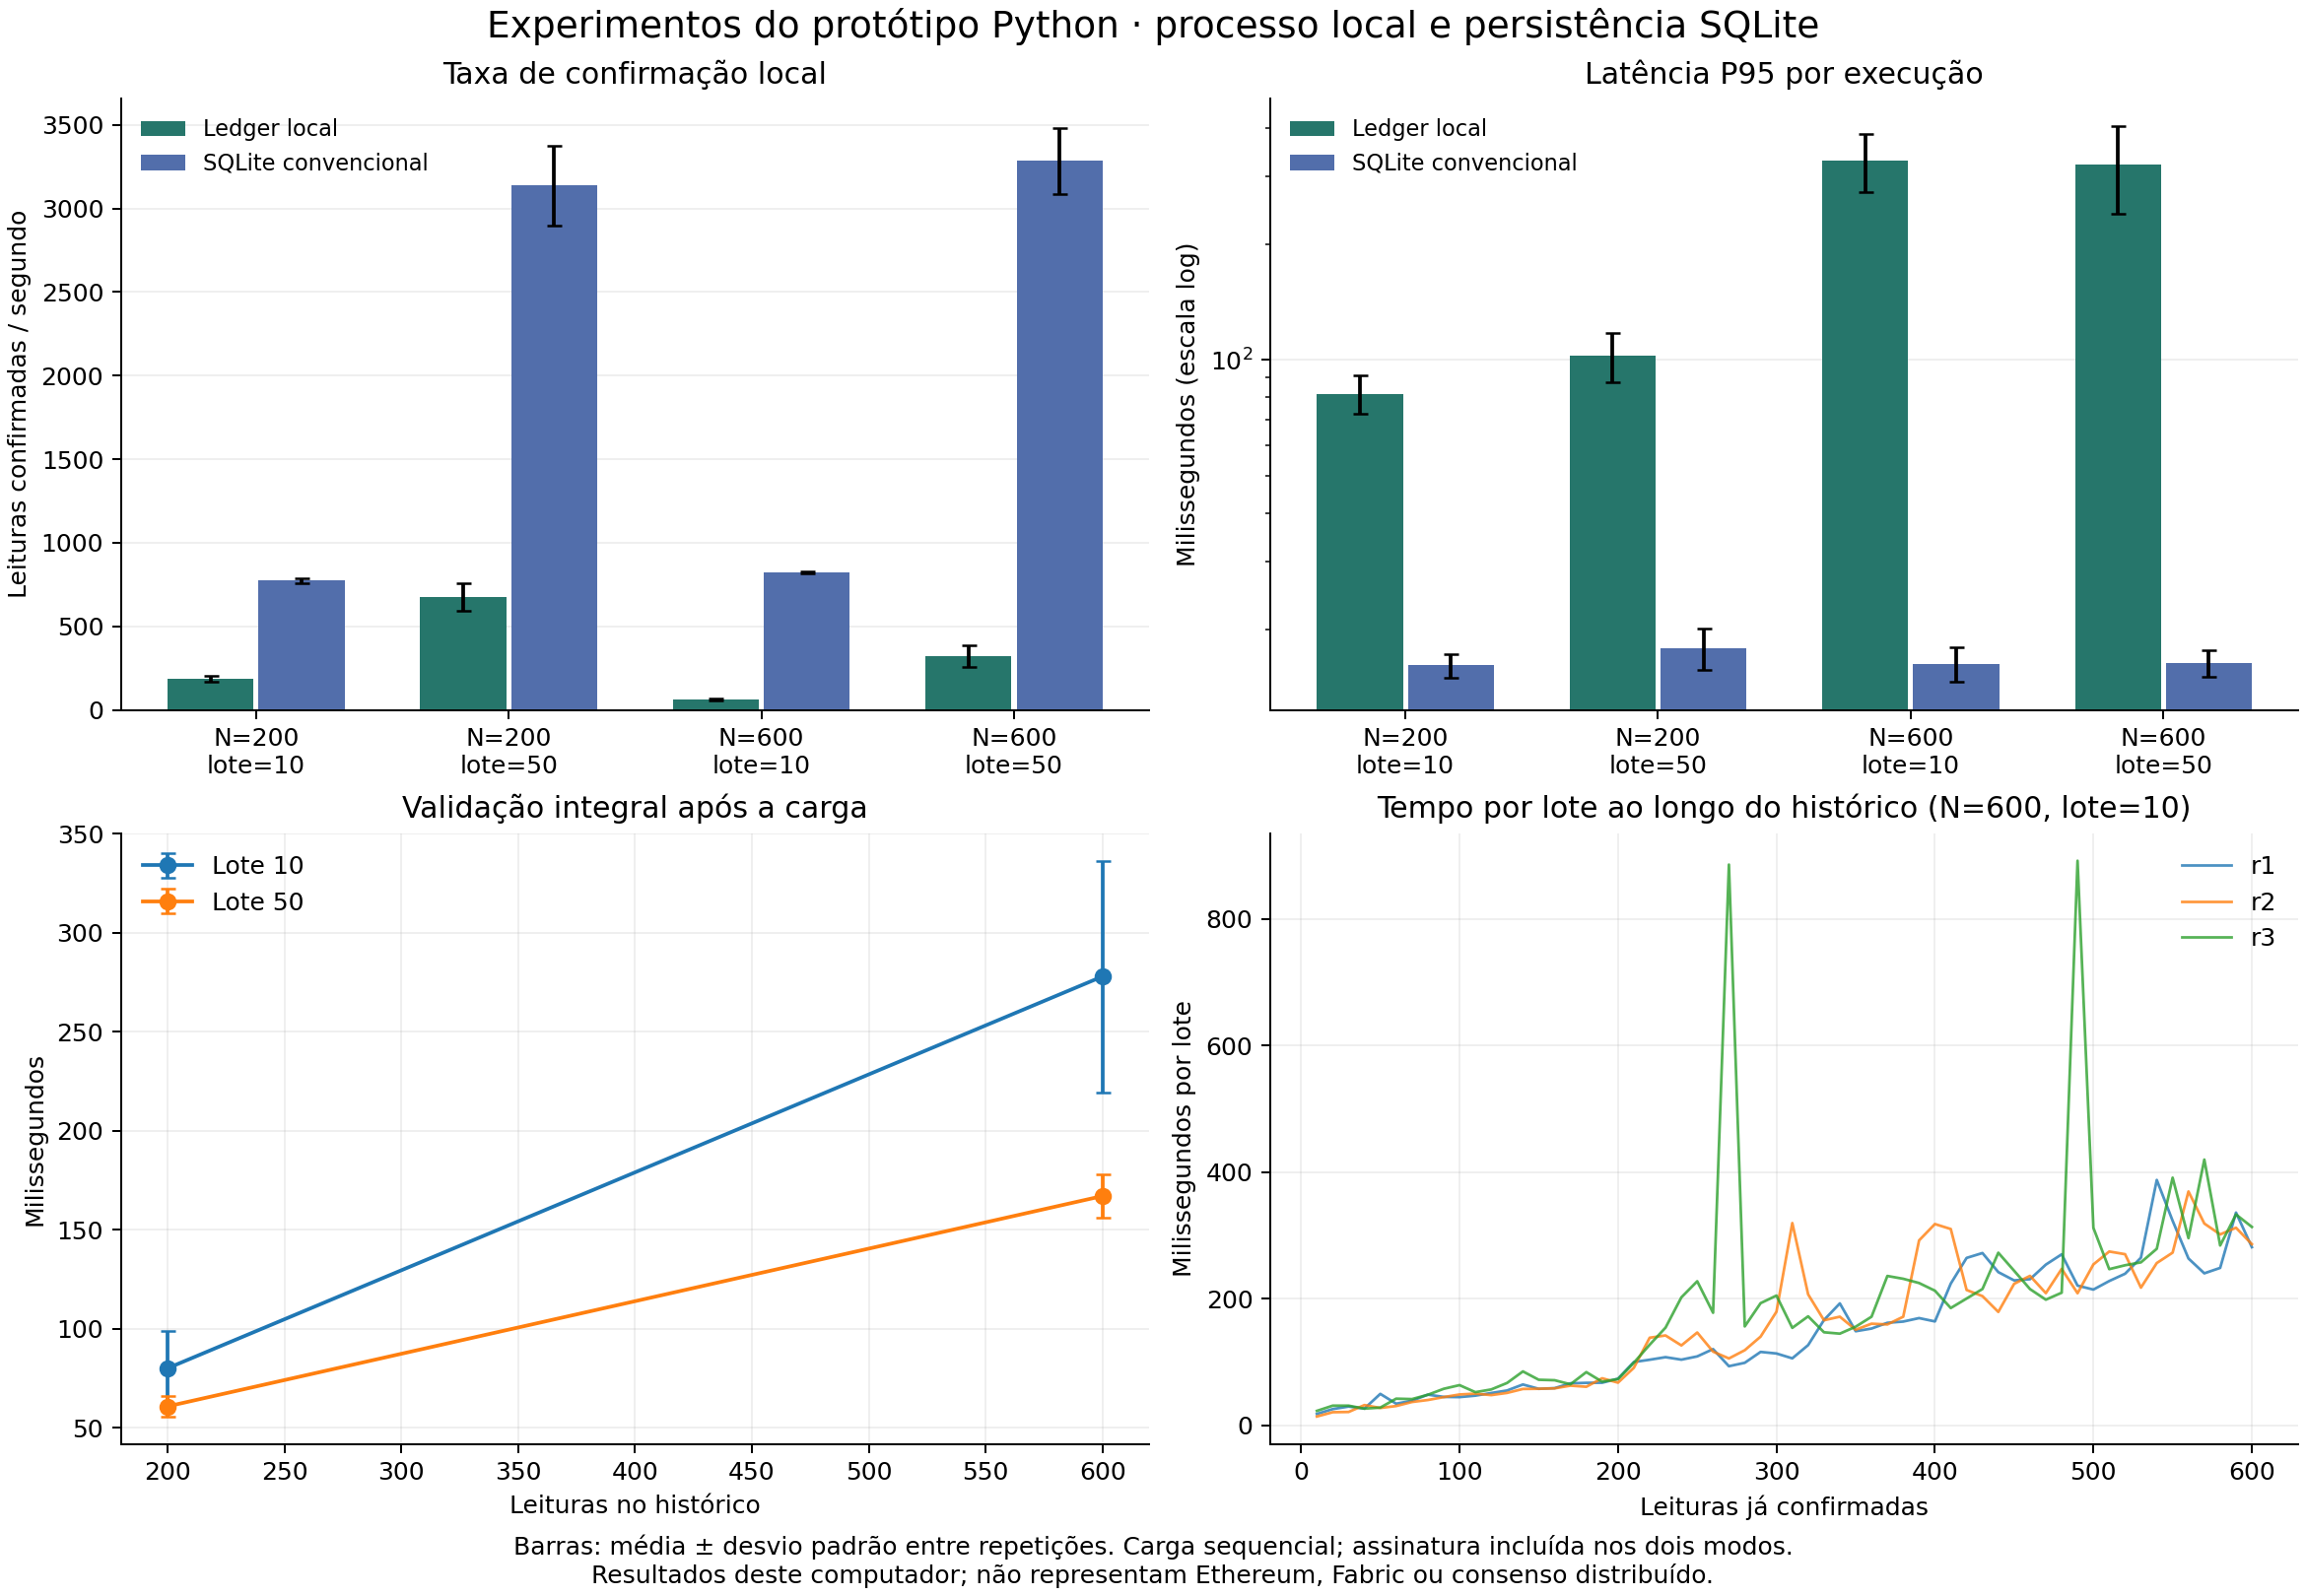
\includegraphics[width=0.92\textwidth]{figura_desempenho.png}
\caption{Taxa de confirmação, P95, validação final e duração dos lotes na coleta local arquivada. Não representa Ethereum, Hyperledger Fabric ou consenso distribuído.}
\label{fig:desempenho}
\end{figure*}

O tempo de CPU médio variou de 0,229 a 7,120 s no ledger e de 0,042 a 0,302 s no controle. O pico do processo variou de 31,75 a 33,09 MiB no ledger e de 31,53 a 32,83 MiB no controle, incluindo imports, preparação e recuperação; não é memória incremental da carga. O tamanho lógico dos bancos não mede diretamente o custo das garantias criptográficas. Os números foram extraídos de \texttt{resultados/execucao-final/resumo.csv}; as 24 execuções e fontes medidas estão preservadas com a distribuição.

\subsection{Comparação bibliográfica entre plataformas}
A literatura indica que os resultados de desempenho variam de acordo com arquitetura, configuração, carga e ambiente experimental. O estudo de Pajooh et al. avalia uma implantação do Fabric em testbed IoT, enquanto Androulaki et al. descrevem a arquitetura do Fabric e não devem ser tratados como se fornecessem uma única métrica universal de TPS \cite{Pajooh2022,Androulaki2018}. Estudos comparativos entre Fabric e Ethereum privado também precisam ser distinguidos de medições da rede pública Ethereum \cite{Khan2025}.

Os valores quantitativos retirados da literatura devem ser mantidos acompanhados da fonte, configuração experimental, tipo de rede e definição da métrica. Quando essas informações não puderem ser verificadas, é preferível apresentar o achado de forma qualitativa ou excluir o número em vez de sugerir uma comparação controlada inexistente.


A evidência disponível deve ser lida em três níveis distintos. O primeiro é o comportamento da rede pública Ethereum, cuja segurança decorre do protocolo aberto de PoS e cujo custo e latência são influenciados pelas condições da rede. O segundo é o comportamento de redes permissionadas construídas com Ethereum/Geth, que não necessariamente reproduzem as condições de participação e o modelo de finalidade da mainnet. O terceiro é o desempenho do Fabric, cuja arquitetura modular permite ajustar endosso, orderers, peers, tamanho de bloco, canais e políticas. Comparar resultados entre esses níveis sem explicar as diferenças mistura efeitos de plataforma com efeitos de configuração.

Na configuração de um host estudada por Pajooh et al., a latência média permaneceu abaixo de um segundo até uma carga próxima de 100 TPS; cargas maiores elevaram a latência e expuseram gargalos de validação. Em Khan et al., a comparação entre Fabric e Ethereum privada apontou vantagem de até cinco vezes no throughput e até 26 vezes na latência para algumas funções de invocação, mas a Ethereum privada apresentou desempenho superior em consultas específicas. Esses valores são úteis como evidência de que o tipo de operação e a configuração importam; não servem como estimativa direta do desempenho do protótipo Python, que é monoprocesso, nem como ranking universal de redes públicas e privadas \cite{Pajooh2022,Khan2025}.

\begin{table*}[t]
\centering\small
\caption{Evidências de desempenho na literatura e limites de interpretação.}
\label{tab:literatura-desempenho}
\begin{tabularx}{\textwidth}{p{0.23\textwidth}p{0.27\textwidth}p{0.24\textwidth}X}
\toprule
Estudo & Objeto avaliado & Achado reportado & Limite para a comparação deste trabalho \\
\midrule
Pajooh et al. (2022) & Fabric em cenários de um e de múltiplos hosts orientados a IoT. & Na configuração de um host, latência média abaixo de 1 s até cerca de 100 TPS; a validação pode se tornar gargalo com aumento da carga. & O número não se transfere aos cenários distribuídos do estudo nem a outras topologias. \\
Pancari et al. (2023) & Controle de acesso baseado em atributos em Ethereum e Fabric para casa inteligente. & Analisa desenho e adequação de mecanismos ABAC nas duas plataformas. & O resultado está associado ao modelo de autorização implementado; não deve ser interpretado como benchmark universal de TPS. \\
Khan et al. (2025) & Fabric e Ethereum privada/Geth com funções de contrato e múltiplos tamanhos de lote. & Até 5 vezes mais throughput e até 26 vezes menor latência do Fabric em certas funções de invocação; Ethereum privada teve vantagem em consultas específicas. & É uma comparação entre configurações privadas e operações definidas, não entre Fabric e Ethereum pública em todos os cenários. \\
Protótipo deste artigo & Ledger Python local e controle SQLite, com leituras simuladas. & 113 testes funcionais aprovados na distribuição atual; 24 execuções de carga arquivadas. & Modos com garantias distintas; HTTP, sensores físicos e redes distribuídas não foram medidos. \\
\bottomrule
\end{tabularx}
\end{table*}


\section{O problema do oráculo em aplicações IoT}
A blockchain pode preservar um registro depois de incorporado ao ledger e, ao mesmo tempo, preservar fielmente um dado errado. Esse limite surge porque o protocolo verifica a validade da transação conforme regras computacionais, mas não observa diretamente o fenômeno físico que originou a informação. Um sensor pode estar mal calibrado, danificado, instalado em local inadequado, sob controle de um invasor ou executar firmware comprometido. Um dispositivo autorizado também pode enviar deliberadamente uma leitura incorreta. A assinatura confirma que o conteúdo foi produzido por uma chave privada correspondente à identidade cadastrada; não comprova que a leitura represente corretamente a temperatura, pressão, posição ou outra variável real \cite{Christidis2016,Yaga2018}.

O teste de oráculo do protótipo torna o problema explícito: a leitura de valor \texttt{999.9}, embora extrema para o cenário de temperatura usado, é aceita quando é assinada pela identidade autorizada. Isso não constitui falha no teste, pois o comportamento esperado do algoritmo de assinatura é verificar autoria e integridade da mensagem, não executar validação física contextual. Para rejeitar o valor, o sistema precisaria de uma regra complementar que conhecesse a variável medida, sua unidade, a faixa plausível, o estado de calibração e a política de exceções. Mesmo um limite fixo pode rejeitar leituras legítimas em condições ambientais excepcionais, de modo que tais regras devem ser validadas com especialistas do domínio.

Há diferentes camadas de mitigação. Na camada física, calibração, sensores redundantes e manutenção reduzem a probabilidade de erros não intencionais. Na camada de dispositivo, inicialização segura, atualização autenticada, proteção de chaves e atestação de firmware podem reduzir alguns riscos de comprometimento. Na camada de dados, verificações de faixa, comparação entre fontes, detecção estatística de outliers e associação de metadados de qualidade podem classificar leituras antes da persistência. Na camada de governança, múltiplas organizações podem atestar resultados ou operar oráculos independentes. Nenhuma medida é universal: redundância não resolve falhas correlacionadas, e um conjunto de fontes pode compartilhar o mesmo erro de calibração ou a mesma origem comprometida.

Uma arquitetura robusta também deve distinguir estados diferentes do dado. Por exemplo, uma leitura pode ser registrada como recebida, validada sintaticamente, validada por regra física, contestada ou corrigida por evento posterior. Como os registros já gravados não devem ser silenciosamente sobrescritos, correções podem ser representadas por novos eventos que indiquem a referência ao registro original, o motivo da correção e a identidade do responsável. Esse padrão melhora a auditabilidade, mas deve ser combinado com regras de retenção e minimização de dados.

\subsection{Dados brutos, hashes e armazenamento fora da cadeia}
Registrar cada leitura bruta on-chain oferece verificabilidade, mas aumenta custo e exposição de dados. Guardar os dados detalhados fora da cadeia e incluir apenas um hash ou referência pode reduzir esse problema; a auditoria compara o dado recuperado com o hash publicado para verificar se corresponde à versão ancorada. A estratégia depende da disponibilidade e da retenção do repositório externo: se os dados brutos forem apagados ou perderem-se, o hash isolado não os reconstrói. Além disso, um hash previsível pode permitir ataques de dicionário ou correlação quando o universo de valores possíveis é pequeno. Assim, off-chain não é sinônimo de anonimização e deve ser projetado com análise de risco.

\section{Discussão}
A comparação entre Ethereum e Hyperledger Fabric deve ser interpretada em função dos requisitos da aplicação. A Ethereum pública pode ser pertinente quando a verificabilidade aberta e a participação ampla são requisitos importantes; uma rede permissionada como o Fabric pode ser mais adequada quando a governança exige identidade conhecida, políticas organizacionais e controle sobre a exposição dos dados. Essa distinção não implica superioridade absoluta de uma plataforma.


A decisão deve considerar o custo total de operação, e não apenas o tempo de confirmação de uma transação. Na rede pública, taxas, auditoria independente e ausência de cadastro prévio podem ser partes centrais do caso de uso. Em uma rede permissionada, a organização precisa financiar e administrar infraestrutura, certificados, atualizações, políticas de endosso, backup, monitoramento e recuperação. A ausência de um token nativo obrigatório não elimina custos operacionais; apenas altera sua natureza e sua distribuição entre os participantes.

A tabela comparativa da Seção de fundamentação não representa uma avaliação empírica feita em condições idênticas. A contribuição é analítica: evidenciar que as plataformas priorizam modelos de confiança diferentes. Ethereum é atrativa quando o sistema precisa oferecer verificabilidade pública e execução de contratos em uma rede aberta. Fabric é atrativo quando as organizações precisam controlar quem participa, quais grupos veem determinados dados e quais participantes aprovam mudanças de estado. Se as partes confiam em um único administrador, o ganho de uma blockchain pode ser pequeno frente à complexidade operacional.

\subsection{O que os testes permitem concluir}
Os testes sustentam os comportamentos implementados nos cenários exercitados: verificação de assinaturas e encadeamento, recusa de replay, cadastro versionado, recuperação do histórico confirmado, autorização administrativa e funcionamento da API, do simulador e do painel. A revogação preserva a validade dos registros anteriores. Isso não prova resistência a qualquer adversário, proteção contra roubo de chaves, disponibilidade após falha de nós, conformidade automática com normas de privacidade ou equivalência com Ethereum/Fabric.

\subsection{Caminho entre o protótipo e uma rede distribuída}
As próximas extensões incluem persistência ou tratamento explícito de pendências após reinício, checkpoint externo confiável, instrumentação do custo de cada componente, avaliação concorrente do caminho HTTP e integração com sensores físicos. Uma experiência distribuída exigiria múltiplos nós independentes, protocolo de ordenação e recuperação, tratamento de partições e um novo desenho de avaliação. Para comparar com Ethereum ou Fabric, seria necessária implantação real dessas plataformas sob carga e critérios de confirmação comuns; os resultados bibliográficos não substituem tal experimento.

Em IoT, a arquitetura também depende do volume de mensagens, tolerância à latência, privacidade e confiança em gateways. Assinar e ancorar um valor não garante sua veracidade física. Se as partes aceitam um único administrador, deve-se avaliar se um banco de dados com trilha de auditoria atende aos requisitos com menor custo operacional.

\subsection{Ameaças à validade}
\begin{itemize}
  \item \textbf{Interna:} instrumentação, cache, frequência dinâmica, tarefas de fundo, antivírus e sincronização OneDrive podem afetar a coleta. A alternância dos modos reduz apenas parte do viés de ordem.
  \item \textbf{De construto:} confirmação significa retorno do commit local. Latência inclui a espera no lote, mas não HTTP, painel, sensor físico, descriptografia ou consenso. A memória é o pico do processo completo.
  \item \textbf{Externa:} um computador, dados sintéticos, quatro sensores, três autoridades locais, dois volumes e três repetições por cenário não definem capacidade máxima nem representam uma rede distribuída.
  \item \textbf{De segurança:} os testes cobrem cenários escolhidos, sem prova formal ou avaliação de administrador malicioso com todas as chaves, sistema operacional comprometido e falhas de hardware.
  \item \textbf{Da revisão:} a ausência de diário completo das buscas limita a reprodutibilidade da síntese bibliográfica.
\end{itemize}

\section{Aspectos de privacidade e conformidade}
A imutabilidade de um registro pode entrar em tensão com obrigações de proteção de dados pessoais. A Lei Geral de Proteção de Dados Pessoais prevê direitos dos titulares e condições para eliminação de dados tratados com consentimento, observadas as hipóteses legais aplicáveis \cite{LGPD2018}. O Regulamento Geral sobre a Proteção de Dados da União Europeia também prevê o direito ao apagamento e exceções específicas \cite{GDPR2016}. Não se deve concluir que todo uso de blockchain seja automaticamente incompatível com essas normas; a avaliação depende do tratamento, da finalidade, da base legal, dos papéis dos agentes e dos dados registrados.

Uma abordagem arquitetural possível é manter dados pessoais detalhados fora da cadeia e registrar apenas referências ou hashes, com controles de acesso adequados. Essa estratégia reduz certos riscos, mas não garante anonimização nem conformidade por si só. A análise jurídica definitiva deve considerar o contexto real da aplicação e, quando necessário, orientação especializada.


Em aplicações IoT, dados aparentemente técnicos podem ser pessoais quando permitem identificar alguém direta ou indiretamente ou inferir hábitos e presença. Leituras de consumo energético, localização, acesso físico, ocupação de ambientes e dados biométricos podem adquirir esse caráter conforme o contexto e a possibilidade de associação. A decisão sobre o que gravar precisa começar por um inventário dos dados, suas finalidades, bases legais, agentes responsáveis, compartilhamentos, prazo de retenção e hipóteses de eliminação.

A imutabilidade técnica não equivale a uma obrigação legal de manter indefinidamente todos os campos. O sistema pode reduzir dados identificáveis antes de registrar, separar identificadores dos eventos, restringir o acesso aos dados fora da cadeia, definir retenção no repositório externo e documentar procedimentos de retificação ou eliminação quando juridicamente aplicáveis. Hashes e identificadores pseudonimizados também exigem avaliação, pois a ausência de nome explícito não garante que a pessoa não possa ser identificada por correlação. A avaliação de conformidade deve ocorrer desde o desenho do sistema e ser contextualizada; não pode ser inferida apenas pelo uso de uma tecnologia permissionada.

Do ponto de vista operacional, uma rede permissionada precisa definir quem atua como controlador ou operador dos dados, como os participantes respondem a incidentes, quem administra certificados, como se revogam credenciais e como são tratados erros de inserção. Essas decisões de governança são tão importantes quanto o formato de bloco ou a função hash. Em redes públicas, a exposição distribuída do registro pode dificultar mudanças e remoções, o que reforça a necessidade de minimização antes da submissão.

\section{Conclusão}
Este trabalho comparou bibliograficamente Ethereum e Hyperledger Fabric e avaliou um protótipo Python local de integridade e rastreabilidade de leituras IoT. A distribuição atual contém SHA-256, Ed25519, cadastro versionado, chaves cifradas, prevenção de replay, SQLite, API autenticada para administração, simulador e painel. Em 2 de novembro de 2026, 113 testes automatizados foram aprovados na distribuição reorganizada. A execução HTTP confirmou duas leituras sintéticas em um bloco, rejeitou acesso sem token, detectou adulteração em cópia e recuperou o histórico íntegro após reinício.

A coleta quantitativa arquivada, feita sobre fontes preservadas anteriores à reorganização, abrange 24 execuções com 9.600 leituras confirmadas. Nas cargas avaliadas, o throughput do ledger variou com volume e agrupamento e foi menor que o do controle SQLite, que executou menos verificações. As medições não incluem o servidor HTTP, a interface ou redes Ethereum/Fabric, e não foram repetidas após a reorganização do pacote. Sua interpretação depende do ambiente e do critério de commit local documentados.

O sistema permanece em um processo, com autoridades em rodízio, sem replicação nem consenso distribuído. A verificação criptográfica não comprova que um sensor mediu corretamente o fenômeno físico. Trabalhos futuros incluem avaliação concorrente do caminho HTTP, persistência de pendências ou tratamento de retomada, checkpoint externo, instrumentação por componente, sensores físicos e, em desenho distinto, implantação de múltiplos nós. Integridade, autoria, autorização, rastreabilidade, disponibilidade, consenso e veracidade física exigem evidências próprias e não devem ser confundidos.

\section*{Agradecimentos}
Os autores agradecem à Universidade Católica Dom Bosco pelo suporte institucional ao desenvolvimento deste trabalho.

\clearpage\balance\bibliographystyle{plainnat}
\bibliography{references}

\end{document}
